\def\year{2018}\relax
%File: formatting-instruction.tex
\documentclass[letterpaper]{article} %DO NOT CHANGE THIS
\usepackage{aaai18}  %Required
\usepackage{times}  %Required
\usepackage{helvet}  %Required
\usepackage{courier}  %Required
\usepackage{url}  %Required
\usepackage{graphicx}  %Required
\frenchspacing  %Required
\setlength{\pdfpagewidth}{8.5in}  %Required
\setlength{\pdfpageheight}{11in}  %Required

\graphicspath{ {./images/} }
%PDF Info Is Required:
  \pdfinfo{
/Title (Heart Disease Classifier)
/Author (AAAI Press Staff)}
\setcounter{secnumdepth}{0}  
 \begin{document}
% The file aaai.sty is the style file for AAAI Press 
% proceedings, working notes, and technical reports.
%
\title{Heart Disease Classifier}
\author{Group 18\&X: Zhong Yuyi, Li Denhao, Li Bo, Zhang Junda, Zhu Leyan, Mao Yancan\\
Zhong Yuyi: leader and train Dataset2 in Logistic Regression model\\
Li Denhao: data process, train dataset3 in LSTM and dataset2 in XGboost\\
Li Bo: data process, train dataset1 in logsitic regression and dataset2 in Naive Bayes\\
Zhang Junda: visulization and front-end implementation\\
Zhu Leyan: train dataset2 in SVM \\
Mao Yancan: data process, train dataset1 in XGboost, SVM, naive bayes and Neural Network\\
}
\maketitle
\begin{abstract}
AAAI creates proceedings, working notes, and technical reports directly from electronic source furnished by the authors. To ensure that all papers in the publication have a uniform appearance, authors must adhere to the following instructions. 
\end{abstract}

\section{Introduction}
Health is always the most concerned topic of people. A statistical data collected from more than 190 countries shows that every year 17.3 million deaths are related with heart disease, which remains the No. 1 global cause of death (Heart Disease and Stroke Statistics — 2015). According to a study, Singaporeans suffer heart failure about 10 years earlier than Americans and Europeans, and nearly 1 in 3 Singaporeans are dying from heart disease. In order to increase the average health standard for Singaporeans, one of the best way is to examine people’s heart condition early and find the pathogeny accurately.
In this report we are going to introduce an application which can help analysing and predicting the heart disease in two specific aspects: Cardiac Arrhythmia and Cardiovascular diseases. We first collect the basic information about patients such as age, gender, resting blood pressure and so on give a general diagnosis (first step). Then we will further examine the heart rhythm (second step) and heart sounds (third step) of patients. The diagnosis of heart rhythm is classified into 13 classes and diagnosis of heart sounds is classified into 3 classes. Based on these 3 steps and detailed classifications, doctors can have more confidence to give a accurate analysis result, which also help curing patients correctly and effectively.
 
To achieve this goal we use 3 datasets, one dataset for each step. The first dataset dates from 1988 and consists of four databases: Cleveland, Hungary, Switzerland, and Long Beach VA. Each database provides 76 attributes, including the predicted attribute. The second dataset are based on the Electrocardiogram (ECG) readings and other attributes. There are 279 attributes in total and grouped into 5 blocks: features concerning biographical characteristics, features concerning average wave durations of each interval, features concerning vector angles of each wave, features concerning widths of each wave and features concerning amplitudes of each wave. The third dataset are all WAV files gathered from two sources: (A) from the general public via the iStethoscope Pro iPhone app, provided in Dataset A, and (B) from a clinic trial in hospitals using the digital stethoscope DigiScope, provided in Dataset B. Some of the attributes value are missing in these three datasets, so we do some pre-handling process with each dataset. After comparing different machine learning models and adjusting parameters related, we use Gradient Boosting Decision Tree (GBDT) for the first and second datasets, and Long Short-Term Memory (LSTM) for the third dataset because of their good performance.


\section{Model In Application}

\section{Application Implementation}

\subsection{Model Description}

\subsubsection{LSTM}

Long Short-Term Memory is a variant of recurrent neural network, which uses special units that can maintain information in memory for long periods of time in addition to standard units, which allows for a better control over the gradient flow and enable better preservation of “long-range dependencies”. The key point for implementing LSTM is to figure out what to forget, save and ignore as a memory cell. Since LSTM is a state-of-art deep learning method and has been widely used on different topics with great performance, we picked this model to see how it works for our application.


\subsubsection{GBDT}

Gradient boosting is a machine learning technique for regression, classification and sorting tasks. It belongs to boosting algorithm family, which can enhance a weak learner to a strong learner. Boosting algorithms are based on the idea that it?s better to get a result by synthesizing many experts? judgements than getting it from only one of them. Gradient boosting, same as other boosting algorithms, constructs the final prediction model with an ensemble of many weak learners, usually decision tree. This is what we call Gradient Boosting Decision Tree(GBDT).

Boosting is one of the major methods of ensemble learning. It constructs model using a stage-wise iterative method. The weak learner constructed at every step of iteration is designed to make up for the deficiency of the existing model. Gradient boosting does it by construct a learner that reduces the loss along the steepest gradient in each step. Gradient boosting has an enormous scope of application since it is capable of processing all kinds of learning tasks by setting different loss functions. It can resist noise in training data effectively as well.

Gradient boosting algorithm tends to use decision tree because this algorithm is easy to understand and has strong interpretability and rapid forecasting speed. Also, decision tree algorithm can process data with missing fields well and do not need to consider interdependence between features.

According to above, Gradient Boosting Decision Tree is one of the best, state-of-the-art machine learning algorithms. Therefore, we choose it for our first two datasets.

\subsection{Application Training result}

\subsubsection{UCI Dataset Result}

There are many missing attribute values in UCI dataset. In addition, the Cleveland data set became corrupted after the loss of a computing node, and the surviving data set contains only 14 attributes per instance(shown at Figure \ref{fig:dataset-1}). Therefore, we constructed a 14 attributes UCI dataset with 920 instances, and the last row ("num") is the attribute to be predicted. In these instances, some of them also have unobserved attributes, for all of unobserved attributes, we replaced them to a certain number "-69" which means unobserved, and we divide the whole dataset into training data and test data with a proportion of 4:1. All model used in UCI dataset will use this processed dataset.

\begin{figure}[!htbp]
\centering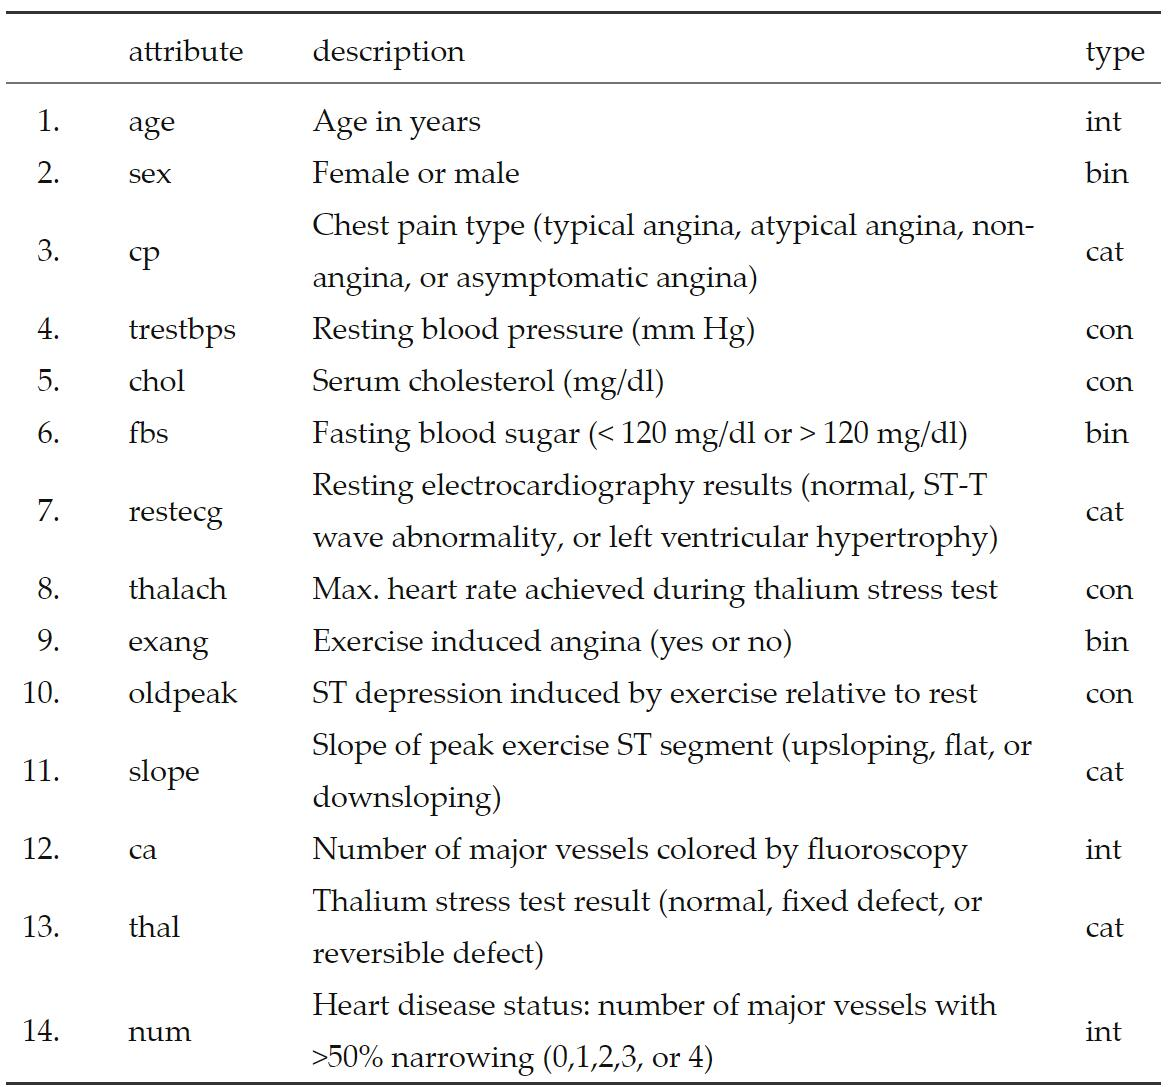
\includegraphics[width=0.4\textwidth]{dataset-1}
\caption{Attributes}
\label{fig:dataset-1}
\end{figure}
UCI dataset was used at the first step of our application, it provides basic information. Because UCI dataset's attributes are limited and could be commonly measured, our application uses UCI dataset to train a general classifier. We have trained it with five models, they are GBDT in LightGBM, Naive Bayes, SVM, Neural Network and Logistic Regression. After comparing the accuracy between these models with tried every model's best performance in this dataset(will be shown in next chapter) and every member of our group developed one of models in this dataset. Finally we found that GBDT had highest and stable accuracy about 89.57\%. As a result, we chose LightGBM as our final training library. LightGBM is efficient, low memory usage and better accuracy with a gradient boosting method. Additionally, LightGBM can be used for nearly all regression problems, our classifier is exactly one of them.

In LightGBM, we have taken a lot of time in reading the documentation and trying to understand the principle of GBDT, such as what is gradient and boosting. Besides, when using default parameters in LightGBM model, we got an accuracy 82.83\% which is too low. Therefore, we tried to improve the accuracy of model's performance. On the one hand, we eliminated some least important attributes in this model by using Pandas, the importance of every attributes using in LightGBM are shown at Figure \ref{fig:dataset-1-impor}, we attempted to eliminate FBS and RESTECG, but the accuracy dropped, so we didn't modify attributes using this model. On the other hand, we modified LightGBM model's attributes by using a script, this script continuously modifies parameters of model's like number of leaves, minimum data in a leaf, learning rate and so on, then find the parameters result with best accuracy. Finally, we got a optimal result with accuracy 89.57\%.

\begin{figure}[!htbp]
\centering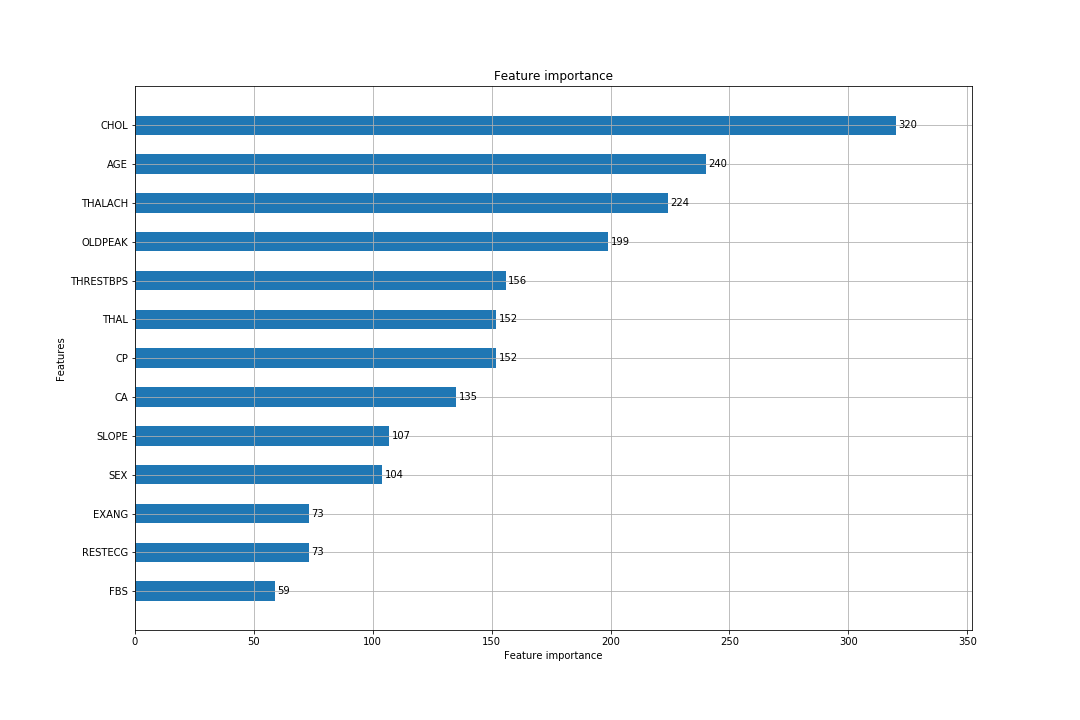
\includegraphics[width=0.5\textwidth]{dataset-1-impor}
\caption{Importance of attributes in LightGBM}
\label{fig:dataset-1-impor}
\end{figure}

\subsubsection{Dataset2 Result}

\subsubsection{Dataset3 Result}

\subsubsection{Most Painful Experience}

\subsection{Application Display}

show the final result of our app.

show some figure of our application.

\section{Experiment}

\subsection{Experiment Setup}
We have pushed our project into Github, and to see more details about our application, you could setup an experiment by yourself. Our project is running as a website. To setup the service, first you should ensure you have installed Anaconda3 and python library LightGBM. Second, you should install front-end framework package Bootstrap and back-end framework package Bottle. Then you could run the service in our repository.

\subsection{Model Comparison}

The information we can derive the heart sound is limited as it is prone to be contaminated by environment noise. Basically, we are able to observe two types of abnormalities in a piece of heart sound: murmur, which indicates the blood reverse flow caused by mitral insufficiency, and extra systole, which indicates myocardial injury. These two kinds of abnormalities are independent, so we extract the starting part of Fourier transform power (frequency lower than 470Hz) and a binary sequence marking the existence of heart beat pulse in 0.075s time interval (about the width of a pulse) as sequential features for murmur heart sound and extra systole respectively. We built two two-layer LSTM model to classify these sequential features. The evaluation of the two models are shown below:

TO BE ADDED

[insert table here]

As explained above, our heart disease testing based on three data sources: biographical information, ECG and heart sound.

We regard biographical information as a vector indicating a sample in the sample space. And for the ECG data, we use the method introduced by Guvenir et al. in \cite{ECG} to extract a 275 dimensional feature for each sample.  For such classification task, we tested four binary classification models: support vector machine (SVM), logistic regression, naïve Bayes and gradient boosting decision tree (GBDT). 
The performance of the four models on dataset1 and dataset2 are shown at Figure \ref{fig:dataset-1-comparison}, we have implemented all of those models into UCI dataset and dataset2(later modify), and the type of UCI dataset and dataset2 are both text(professional word), our process method in processing these two datasets is similar. We will introduce how we get the optimal accuracy of each model.

\begin{figure}[!htbp]
\centering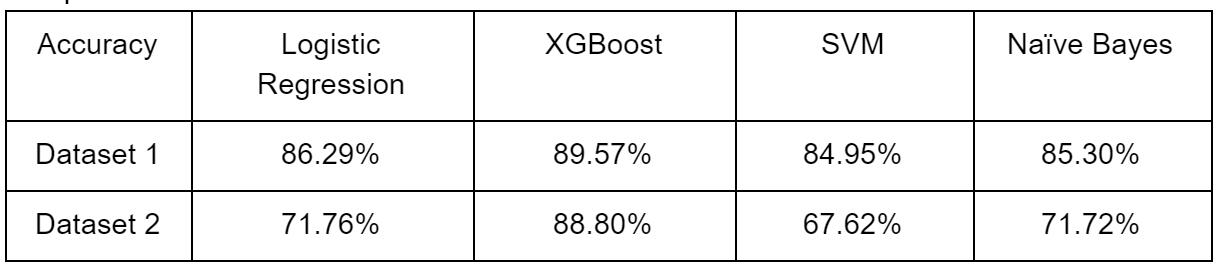
\includegraphics[width=0.4\textwidth]{dataset-1-comparison}
\caption{The result of using different model with optimal attributes}
\label{fig:dataset-1-comparison}
\end{figure}

\subsection{Optimization method}

We used Sklearn to invoke both Logistic Regression, SVM and Naive Bayes models, and logistic regression has the secondly good accuracy in both UCI dataset and dataset2. The optimization method for both of these three method is to select columns to make the cross validation be best. Excepting for select columns method, we also have different method for different models.

\subsection{Logistic Regression Optimization}

For Logistic Regression, we 

\subsection{SVM Optimization}

For SVM, we

\subsection{Naive Bayes Optimization}

For Naive Bayes, we

\section{Conclusion}

We implement an application meant for heart disease detecting, which uses three different aspects including overall healthy condition, cardiac arrhythmia and heartbeat sounds to diagnose the final result step by step. By the end, we obtain relatively reliable performance and provide a platform for other users. It should be noted that we tried several  models on three datasets and picked up the optimal model as the final model for our app. Through this project, we learn how to do demand analysis, performance evaluation and also tuning skill, which helps us to understand further for machine learning.

\section{References}

\end{document}
